\section{Preliminaries}
\label{sec:Preliminaries}
In the whole article $\Z_2$-coefficients for homology and cohomology will be understood,
unless explicitly stated otherwise.

In this section we recollect some classical definitions and results about braid groups and mapping class groups.
Let $\sg$ be a compact, smooth, orientable surface of genus $g$ with one parametrised
boundary component $\partial \sg$. Let $\sgm$ be $\sg$ with a choice of $m$ distinct
points in the interior: these points are called \emph{punctures} and are not assumed to be ordered.

\begin{defn}
\label{defn:cms}
 The $m$-th \emph{ordered configuration space} of a surface $\sg$ is the space
\[
 F_m(\sg)=\set{(P_1,\dots,P_m) \in \pa{\mathring{\Sigma}_{g,1}}^{\times m}  \,|\,  P_i\neq P_j  \;\forall i\neq j}.
\]

 Notice that we require the points of the configuration to lie in the interior of $\sg$;
 $F_m(\sg)$ is a smooth, orientable $2m-$dimensional manifold.
 
 The symmetric group $\mathfrak{S}_m$ acts freely on $F_m(\sg)$ by permuting the points of a configuration;
 the orbit space
 \[
 F_m(\sg)/\mathfrak{S}_m
 \]
 is called the \emph{$m-$th unordered configuration space}
 of $\sg$ and is denoted by $C_m(\sg)$; this space is also a $2m-$dimensional orientable manifold
 (see figure \ref{fig:unordered}).
 
%  
%  We denote by $C_k(\sg)^c$ the one-point compactification of the space $C_k(\sg)$; the point
%  at infinity is denoted by $*$ and serves as basepoint.
\end{defn}

\begin{figure}\centering
 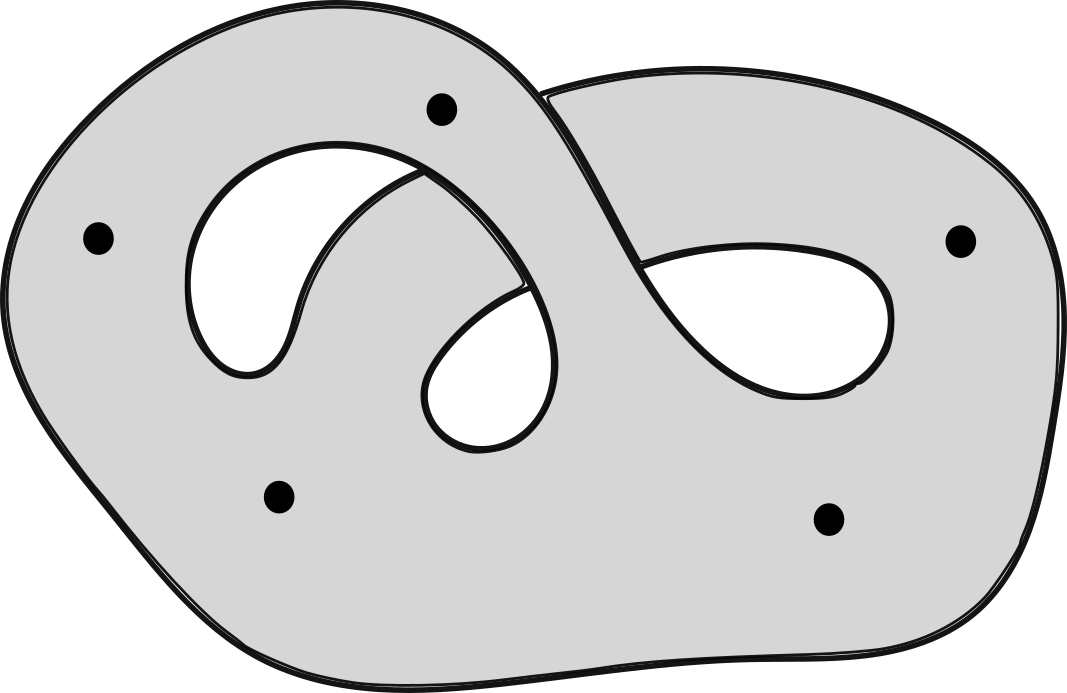
\includegraphics[scale=0.8]{figures/unordered.png}
 \caption{A configuration in the space $C_5(\Sigma_{1,1})$}
\label{fig:unordered}
\end{figure}


A classical result by Fadell and Neuwirth (\cite{FadellNeuwirth}) ensures
that $C_m(\sg)$ is aspherical; the fundamental group $\pi_1(C_m(\sg))$ is
called the \emph{braid group on $m$ strands of $\sg$} and is denoted by $\bms$.

\begin{defn}
 \label{def:mcg}
 Let $\Diff(\sg;\partial\sg)$ be the group of diffeomorphisms of $\sg$ that fix $\partial\sg$ pointwise,
 endowed with the Whitney $C^{\infty}-$topology. We denote by $\gg=\pi_0(\Diff(\sg;\partial\sg))$ its group of connected
 components, which is called the \emph{mapping class group} of $\sg$.
 
 Similarly let $\Diff(\sgm;\partial\sgm)$ be the group of diffeomorphisms of $\sgm$ that fix $\partial(\sg)$
 pointwise and restrict to a permutation of the $m$ punctures, and let $\ggm=\pi_0(\Diff(\sgm;\partial\sgm))$ be its
 group of connected components, called the mapping class group of $\sgm$.
 \end{defn}
 A classical result by Earle and Schatz (\cite{EarleSchatz}) ensures that the connected components
 of $\Diff(\sg)$ are contractible. In particular $B\Diff(\sg;\partial\sg)\simeq B\gg$ is
 a classifying space for
 the group $\gg$, i.e. a space of type $K(\gg,1)$; we call $\cF_{g,1}\to B\Diff(\sg;\partial\sg)$ the universal
 $\sg-$bundle
 \[
  \cF_{g,1}\colon=\sg\times_{\Diff(\sg;\partial\sg)}E\Diff(\sg;\partial\sg)\to B\Diff(\sg;\partial\sg).
 \]
Applying the construction of the $m-$th unordered configuration space fiberwise we obtain a bundle
$C_m(\cF_{g,1})\to B\Diff(\sg;\partial\sg)$ with fiber $C_m(\sg)$.

The space $C_m(\cF_{g,1})$ is a classifying space for the
group $\ggm$ and the Birman exact sequence \ref{eq:Birman} is obtained by taking fundamental
groups of the aspherical spaces
\begin{equation}\label{eq:Birmanbundle}
C_m(\sg)\to C_m(\cF_{g,1})\to B\Diff(\sg;\partial\sg).
\end{equation}

In the whole article the genus $g$ of the surfaces that we consider is supposed to be fixed,
unless explicitly stated otherwise, and we will abbreviate $\S=\sg$.
We denote by $\D$ the open disc $\mathring{\Sigma}_{0,1}$.

It will be useful, for many constructions, to choose an embedding
$\D\hookrightarrow\mrS$ near $\partial\S$ and to replace
$\Diff(\S;\partial\S)$ with its subgroup $\Diff(\S;\partial\S\cup\D)$ of diffeomorphisms
of $\S$ that fix pointwise both $\partial\S$ and $\D$. Saying that $\D$ is embedded
\emph{near $\partial\S$} means that there is a compact subsurface $\S'\subset\S$
such that $\S$ is the boundary connected sum $\S'\natural\bar\D$.
From now on we suppose such an embedding to be fixed and we consider $\D$ as a subspace
of $\mrS$ (see figure \ref{fig:SS'D}). In section \ref{sec:HBraidSurf}, definition \ref{defn:Tsg},
we will specify an embedding $\D\hookrightarrow\mrS$ using a particular model for $\mrS$.

\begin{figure}\centering
 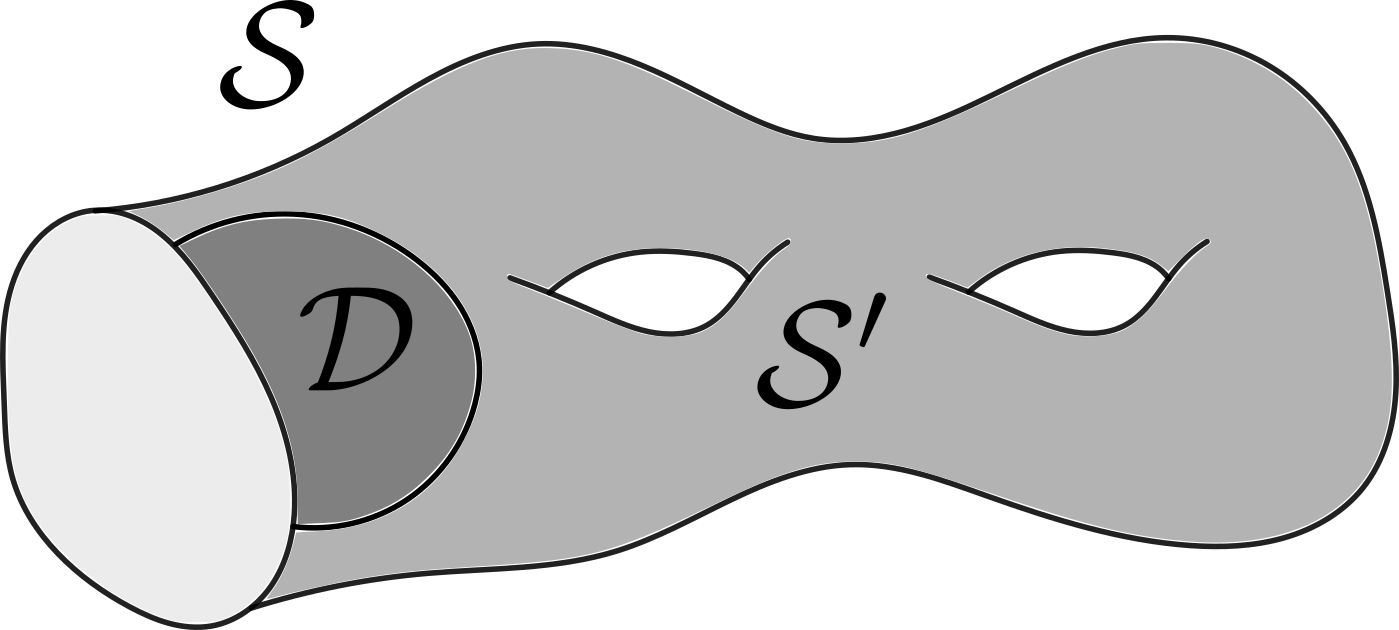
\includegraphics[scale=0.8]{figures/SS'D.png}
 \caption{A splitting of $\S$ as $\S'\natural\bar\D$.}
\label{fig:SS'D}
\end{figure}

The construction of definition \ref{defn:cms} can be specialised to the
surfaces $\D$ and $\S'$, yielding spaces $C_m(\D)$ and $C_m(\S')$ respectively.

The inclusion $\Diff(\S;\partial\S\cup\D)\subset\Diff(\S;\partial\S)$ is a homotopy
equivalence, hence also the induced map
\[
B\Diff(\S;\partial\S\cup\D)\to B\Diff(\S;\partial\S)
\]
is a homotopy equivalence. We will replace the previous construction with the following,
equivalent ones.
\begin{defn}
\label{defn:universalSbundle}
We call $\cF_{\S,\D}\to B\Diff(\S;\partial\S\cup\D)$
the universal $\S-$bundle
 \[
  \cF_{\S,\D}\colon=\S\times_{\Diff(\S;\partial\S\cup\D)}E\Diff(\S;\partial\S\cup\D)\to B\Diff(\S;\partial\S\cup\D).
 \]
Notice that $\Diff(\S;\partial\S\cup\D)$ acts on $\S'$ by restriction of diffeomorphisms, and acts trivially
on $\D$; therefore $\cF_{\S,\D}$ contains subspaces
\[
 \cF_{\S'}= \S'\times_{\Diff(\S;\partial\S\cup\D)}E\Diff(\S;\partial\S\cup\D)
\]
and $\D\times B\Diff(\S;\partial\S\cup\D)$; these subspaces fiber over $B\Diff(\S;\partial\S\cup\D)$
with fibers $\S'$ and $\D$ respectively.

Applying the construction of the $m-$th unordered configuration space fiberwise, we obtain spaces
$C_m(\cF_{\S,\D})$, $C_m(\cF_{\S'})$ and $C_m(\D)\times B\Diff(\S;\partial\S\cup\D)$,
all fibering over $B\Diff(\S;\partial\S\cup\D)$ with fibers, respectively, $\cms$,
$C_m(\S')$ and $C_m(\D)$.
\end{defn}

\begin{defn}
For all $0\leq p\leq m$ there is a natural map
\[
 \mu\colon C_p(\D)\times C_{m-p}(\S')\to \cms
\]
which takes the union of configurations (see figure \ref{fig:defmu}):
 \[
  \mu\pa{\set{P_1,\dots,P_p};\set{P'_1,\dots,P'_{m-p}}}=\set{P_1,\dots,P_p,P'_1,\dots,P'_{m-p}}\in\cms.
 \]
\begin{figure}\centering
 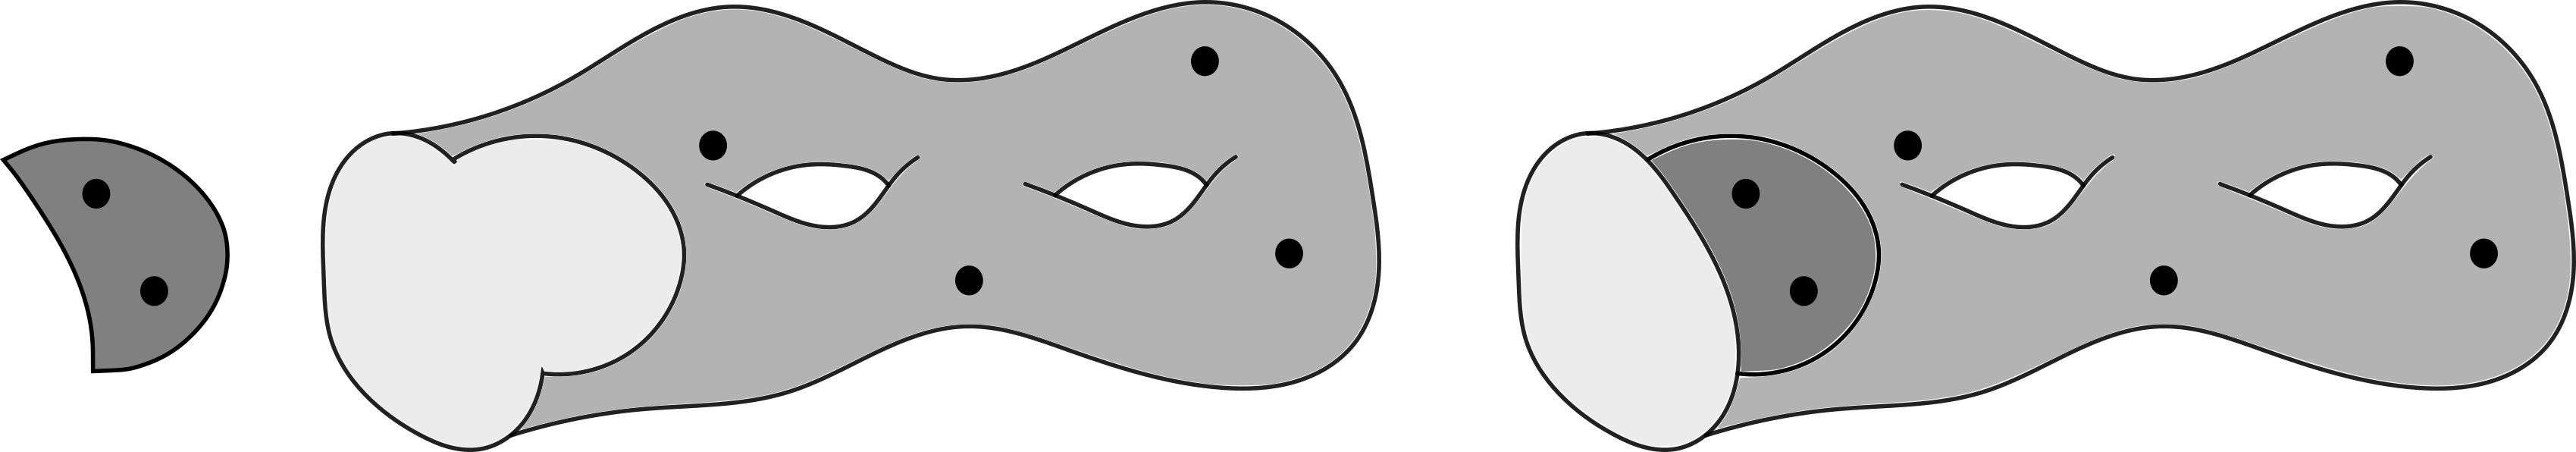
\includegraphics[scale=0.7]{figures/defmu.png}
 \caption{The product of two configurations in $C_2(\D)$ and $C_4(\S)$.}
\label{fig:defmu}
\end{figure}
 
We can apply this construction to each couple of fibers of $C_m(\cF_{\S,\D})$ and $C_{m-p}(\cF_{\S'})$
over the same point of $ B\Diff(\S;\partial\S\cup\D)$, obtaining a map $\mu^{\cF}$:
\[
 \mu^{\cF}\colon C_p(\D)\times C_{m-p}(\cF_{\S'})\to C_m(\cF_{\S,\D}).
\]
If we see the domain of $\mu^{\cF}$ as a fibered product of bundles over $B\Diff(\S;\partial\S\cup\D)$
\[
 \pa{C_m(\D)\times B\Diff(\S;\partial\S\cup\D)}\times_{B\Diff(\S;\partial\S\cup\D)}C_{m-p}(\cF_{\S'}),
\]
then the map $\mu^{\cF}$ is also a map of bundles over $B\Diff(\S;\partial\S\cup\D)$, and the corresponding
map on fibers is precisely $\mu$.
\end{defn}
The fiber bundle \ref{eq:Birmanbundle} corresponding to the Birman exact sequence \ref{eq:Birman}
can now be replaced by the following one
\begin{equation}\label{eq:BirmanbundleD}
\cms\to C_m(\cF_{\S,\D})\to B\Diff(\S;\partial\S\cup\D).
\end{equation}
We conclude this section by recalling the structure of $H_*(C_m(\D))$.

The cohomology of $C_m(\D)$ with coefficients in $\Z_2$ was first computed by Fuchs in
\cite{Fuchs:CohomBraidModtwo}: we will recall this computation in section
\ref{sec:HBraidSurf}, where we will make a similar computation in detail.

In \cite[Chap.III]{CLM} Cohen considers the space $\coprod_{m\geq 0}C_m(\D)$ as an
algebra over the operad of little $2-$cubes, and describes its
$\Z_2-$homology as follows:
\begin{equation}
 \label{eq:Cohen}
H_*\pa{\coprod_{m\geq 0}C_m(\D)}\simeq \Z_2\left[Q^j\epsilon \, |\, j\geq 0\right].
\end{equation}

Here $\epsilon\in H_0(C_1(\D))$ is the fundamental class, and for all
$k,m\geq 0$ we denote by $Q\colon H_k(C_m(\D))\to H_{2k+1}(C_{2m}(\D))$
the first Dyer-Lashof operation. In particular $Q^j\epsilon$ is the generator of
$H_{2^j-1}(C_{2^j}(\D))\simeq\Z_2$. See figure \ref{fig:monomial}

The isomorphism in equation \ref{eq:Cohen} is
an isomorphism of bigraded rings. The left-hand side is a ring with the Pontryagin product
coming from the action of the little $2-$cubes,
and the right-hand side is a polynomial ring in infinitely many variables $\epsilon,Q\epsilon,Q^2\epsilon,\dots$.
The bidegree is given by the homological degree
$*$, that we simply call the \emph{degree},
and by the index $m$ of the connected component
on which the homology class is supported (informally, the number of points
involved in the construction of a homology class), that we call the \emph{weight}.

 \begin{figure}\centering
 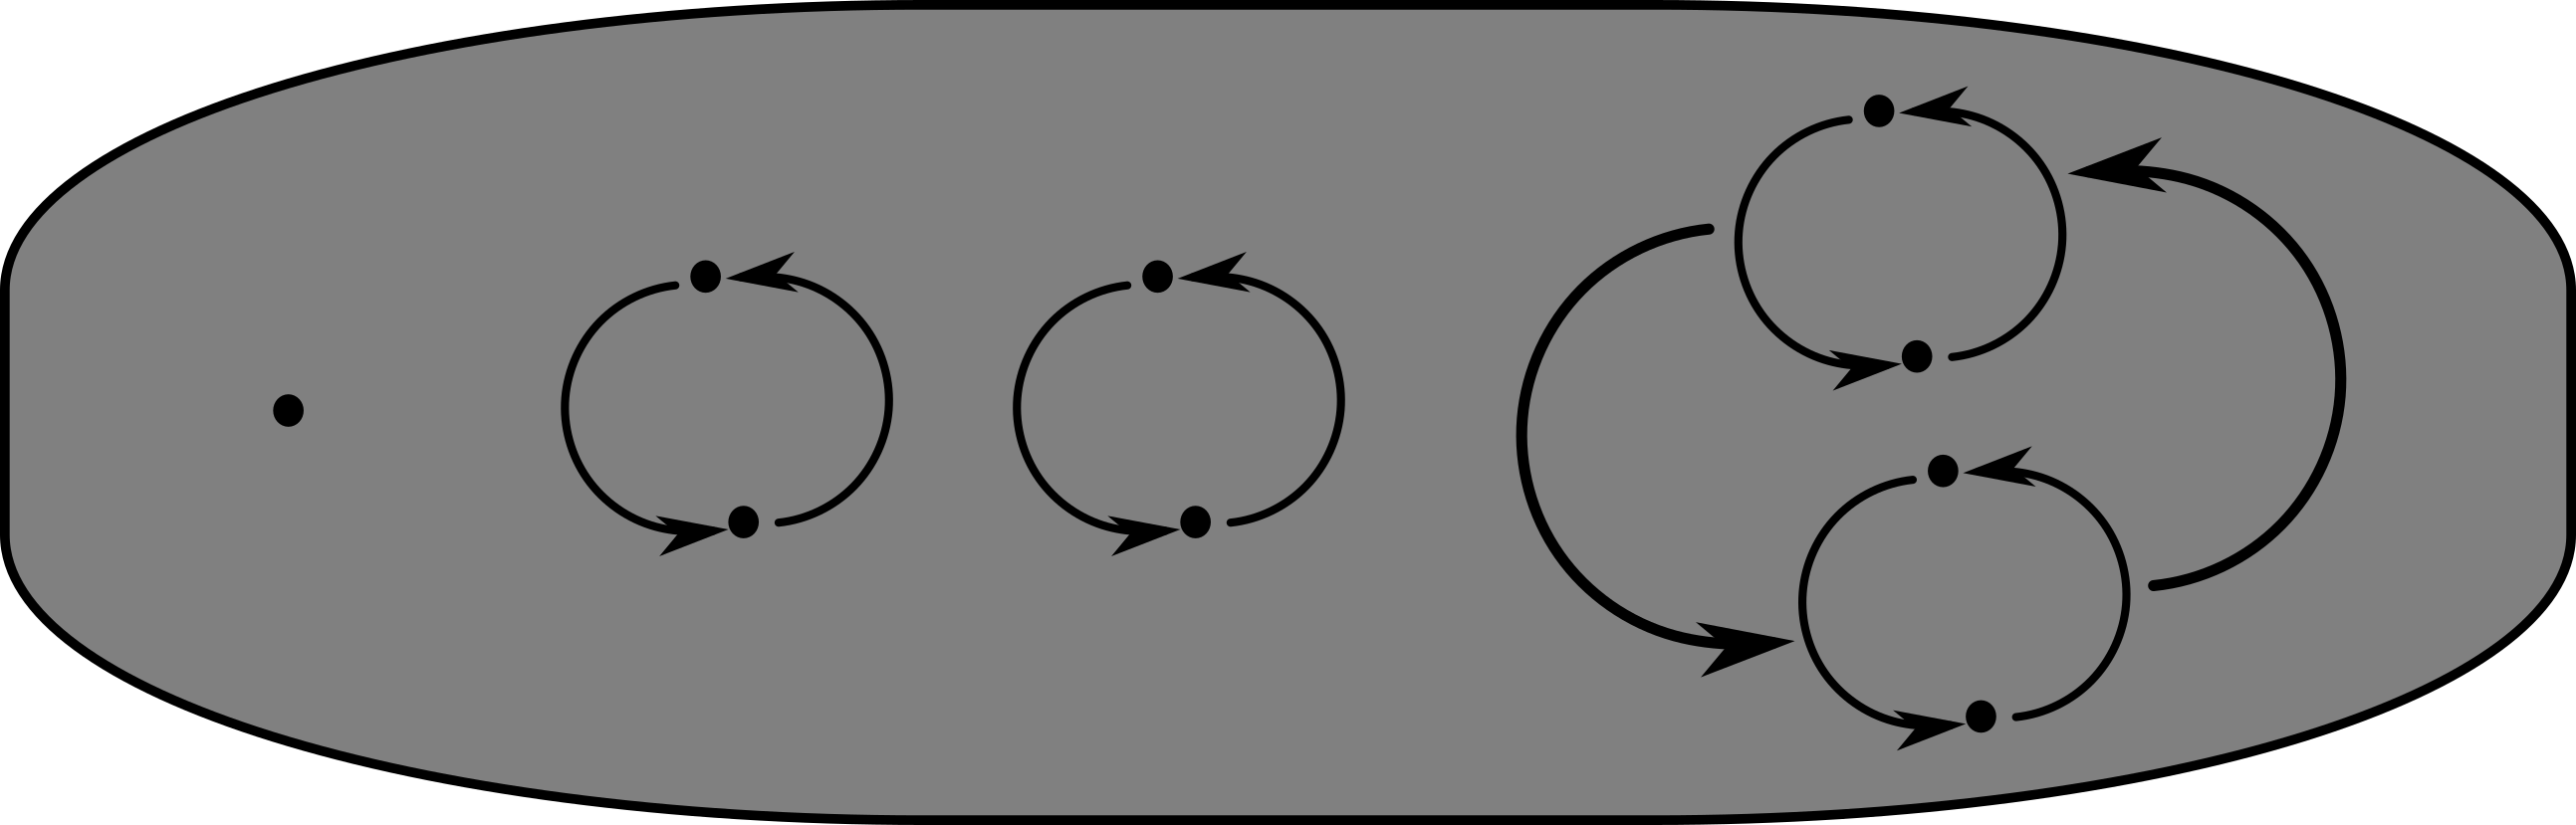
\includegraphics[scale=0.7]{figures/monomial.png}
 \caption{The class in $H_5(C_9(\D))$ corresponding to the monomial $\epsilon\cdot(Q\epsilon)^2\cdot Q^2\epsilon$.}
\label{fig:monomial}
\end{figure}

In this article we will only need the isomorphism in equation \ref{eq:Cohen} to hold as
an isomorphism of bigraded $\Z_2-$vector spaces.
In particular for all choices of natural numbers $(\alpha_j)_{j\geq 0}$ with all but finitely
many $\alpha_j=0$, we will consider the monomial $\prod_j\pa{Q^j\epsilon}^{\alpha_j}$, corresponding to
a homology class in some bidegree $(*,m)$: all that
we are going to need is that the set of these monomials is a bigraded basis for the
left-hand side of equation \ref{eq:Cohen}.